\subsection{tansig}

\noindent
I solved all of my real life problems with this transfer function if a non-linear function was used. In [4] page 2-6 the tansig is defined as in equation \eqref{equ:tansigTransferFunction}. A look on the MathWorks homepage with the keyword tansig will show that tansig is programed as in equation \eqref{equ:tansigTransferFunctionNnet}.

\begin{equation}
	a = \frac{e^n - e^{-n}}{e^n + e^{-n}}
	\label{equ:tansigTransferFunction}
\end{equation}

\begin{equation}
	a = \frac{2}{(1 + e^{-2*n})-1}
	\label{equ:tansigTransferFunctionNnet}
\end{equation}


\begin{figure}[htb]
\centering
  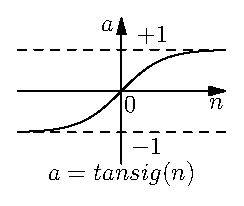
\includegraphics{octave/neuroPackage/graphics/tansig}
\caption{Tansig transfer function}
\label{fig:tansigTransferFunction}
\end{figure}

\begin{figure}[htb]
\centering
  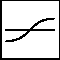
\includegraphics{octave/neuroPackage/graphics/tansiglogo}
\caption{Tansig transfer function logo}
\label{fig:tansigTransferFunctionLogo}
\end{figure}
